\chapter{Appendice}
In questa sezione verranno approfondite alcune funzioni di CPLEX necessarie alle implementazioni descritte nei capitoli precedenti.
\section{Funzioni}
\subsection{Costruzione modello}
Per poter costruire il modello da analizzare, come prima cosa, è necessario creare un puntatore alle due strutture dati utilizzate da CPLEX.
\lstinputlisting[caption={\footnotesize{modelTSP.txt}}, style=code, firstnumber=1, firstline=27, lastline=29, label=tsp_model, language=c]{Source/modelTSP.txt}
La funzione alla riga 2 alloca la memoria necessaria e riempie la struttura con valori di default. Nel caso in cui non termini con successo memorizza un codice d'errore in \textit{\&error}.\\
La funziona invocata nella riga successiva, invece, associa la struttura LP all'ENV che gli viene fornito. Il terzo parametro passato, nell'esempio "TSP", sarà il nome del modello creato.
Al termine di queste operazioni verrà quindi creato un modello vuoto. All'interno del nostro programma per inizializzarlo è stata costruita la seguente funzione:
\begin{center}
\begin{tabular}{c}
\begin{lstlisting}[linewidth=320pt, basicstyle=\footnotesize\sffamily,] 
void cplex_build_model(istanza_problema, env , lv);
\end{lstlisting}
\end{tabular}
\end{center}
\begin{table}[h]
\centering
\begin{tabular}{rl}
\textbf{istanza\_problema: } & {puntatore alla struttura che contiene} \\
&  {l'istanza del problema (letta dal file TSPlib)} \\
\textbf{env: } & {puntatore di tipo CPXENVptr alla}\\
& {struttura ENV precedentemente creata}\\
\textbf{lp: } & {puntatore di tipo CPXLPptr alla}\\
& {struttura LP  precedentemente creata}\\
\end{tabular}
\end{table}
All'interno di \textbf{cplex\_build\_model()} viene aggiunta una colonna alla volta al modello, definendo quindi anche la funzione obiettivo. Le variabili aggiunte corrispondono agli archi del grafo e per ciascuno di questi viene calcolato il costo come distanza euclidea. La funzione necessaria ad inserire colonne e definire la funzione di costo è la seguente:
\vspace{0.5cm}
\begin{center}
\begin{tabular}{c}
\begin{lstlisting}[linewidth=350pt, basicstyle=\footnotesize\sffamily,]     
CPXnewcols(env, lp, num_colonne, costi, lower_bound, 
           upper_bound, tipi_variabili, nomi_variabili);
\end{lstlisting}
\end{tabular}
\end{center}
\begin{table}[h]
\begin{tabular}{rl}
\textbf{env:} & {puntatore di tipo CPXENVptr alla}\\
& {struttura ENV precedentemente creata} \\
\textbf{lp:} & {di tipo CPXLPptr, è un puntatore alla struttura LP}\\
& {precedentemente creata}\\
\textbf{num\_colonne:} & {numero di colonne da inserire} \\    
\textbf{costi:} & {vettore dei costi relativi agli archi da inserire} \\
\textbf{lower\_bound:} & {vettore contenente i lower bound dei valori}\\
& {assumibili dalle variabili da inserire}\\              
\textbf{upper\_bound:} & {vettore contenente gli upper bound dei valori}\\
&  {assumibili dalle variabili da inserire} \\
\textbf{tipi\_variabili:} & {vettore contenente la tipologia delle variabili}\\
& da inserire\\
\textbf{nomi\_variabili:} & {vettore di stringhe contenenti i nomi}\\
& {delle variabili da inserire}
\end{tabular}
\end{table}
La generica colonna \textbf{i}, aggiunta dalla funzione, sarà definita dalle informazioni contenute all'interno della posizione \textbf{i} degli array, ricevuti come parametri. Nel programma elaborato durante il corso, viene aggiunta una colonna alla volta all'interno del modello. Per far ciò, è necessario comunque utilizzare riferimenti alle informazioni da inserire, in modo da ovviare il problema riguardante la tipologia di argomenti richiesti, che sono array. Ad esempio, nel nostro caso, la tipologia di una nuova variabile inserita sarà un riferimento al carattere \textbf{'B'}, che la identifica come binaria.\\
Per poter inserire il primo insieme di vincoli del problema\\
$$
\underset{e\in \delta(v)}\sum{\;x_e} = 2\;\;\;\;\;\;\;\;\;\;\;\;\;\;\;\;\;\;\forall\;v\in V \\\\
$$
\\
viene invece sfruttata la seguente funzione:
\begin{center}
\begin{tabular}{c}
\begin{lstlisting}[linewidth=330pt, basicstyle=\footnotesize\sffamily,]     
 CPXnewrows(env, lp, numero_righe,termini_noti,
            tipi_vincoli, range_valori, nomi_vincoli);
\end{lstlisting}
\end{tabular}
\end{center}
\begin{table}[h]
\begin{tabular}{rl}
\textbf{env:} & {puntatore di tipo CPXENVptr alla struttura ENV}\\
& {precedentemente creata}\\
\textbf{lp:} & {puntatore di tipo CPXLPptr alla struttura LP}\\
& {precedentemente creata}\\
\textbf{numero\_righe:} & {numero di righe (vincoli) da inserire}\\
\textbf{termini\_noti:} & {vettore dei termini noti dei vincoli}\\
\textbf{tipi\_vincoli:} & {vettore di caratteri che specifica il tipo di vincoli}\\
&{da inserire. Ogni carattere può assumere:}\\
&{\textit{'L'} per vincolo $\leq$}\\
&{\textit{'E'} per vincolo $=$}\\
&{\textit{'G'} per vincolo $\geq$}\\
&{\textit{'R'} per vincolo definito in un intervallo}\\
\textbf{range\_valori:} & {vettore di range per i valori di ogni vincolo}\\
& {(nel nostro caso è NULL)} \\
\textbf{nomi\_vincoli} & vettore di stringhe contenenti i nomi  \\
                  & delle variabili da inserire
\end{tabular}
\end{table}
In modo analogo all'inserimento delle colonne, nel nostro programma viene aggiunta una riga alla volta nel modello. L'\textbf{i}-esima riga aggiunta corrisponderà al vincolo imposto sul nodo \textbf{i}-esimo, imponendo a 1 il coefficiente della variabile $x_{k,j}$ se $k=i$ $j=i$ per ogni variabile del modello.\\\\
\subsection{Lazy constraints}
Nel caso in cui si voglia sfruttare la possibilità di verificare se è stato rispettato un vincolo, solo al termine della computazione della soluzione, è necessario inserire un "lazy constraint". Per fare ciò viene utilizzata la seguente funzione:
\begin{center}
\begin{tabular}{c}
\begin{lstlisting}[linewidth=380pt, basicstyle=\footnotesize\sffamily,]     
CPXaddlazyconstraints(env, lp, num_vincoli, nnz, 
					termine_costante, tipo_vincolo, posizione_iniziale,
					indici, valori, nome_vincolo);
\end{lstlisting}
\end{tabular}
\end{center}
\begin{table}[h]
\begin{tabular}{rl}
\textbf{env:} & {puntatore di tipo CPXENVptr alla struttura ENV}\\
& {precedentemente creata}\\
\textbf{lp:} & {puntatore di tipo CPXLPptr alla struttura LP}\\
& {precedentemente creata}\\
\textbf{num\_vincoli:} & {numero di vincoli da inserire}\\
\textbf{nnz:} & {vettore con il numeri di variabili per ogni vincolo}\\ 
\textbf{termine\_costante:} & {vettore dei termini noti dei vincoli}\\
\textbf{tipi\_vincoli:} & {vettore di caratteri che specifica il tipo di vincoli}\\
&{da inserire. Ogni carattere può assumere:}\\
&{\textit{'L'} per vincolo $\leq$}\\
&{\textit{'E'} per vincolo $=$}\\
&{\textit{'G'} per vincolo $\geq$}\\
&{\textit{'R'} per vincolo definito in un intervallo}\\
\textbf{posizione\_iniziale:} & {vettore con le posizione iniziali dei coefficienti nei vincoli}\\
\textbf{indici:} & {vettore di vettori contenenti gli indici delle variabili }\\
& {appartenenti al vincolo}\\
\textbf{valori:} & {vettore di vettori con i coefficienti delle variabili del vincolo}\\
\textbf{nome\_vincolo:} & {vettore con i nomi dei vincoli}\\
\end{tabular}
\end{table}
In modo analogo alle due funzioni precedentemente descritte per l'aggiunta di righe e colonne, nel nostro modello viene inserito un vincolo per volta. Per impostare correttamente i coefficienti delle variabili presenti nel vincolo, vengono sfruttati i due array \textit{indici} e \textit{valori}. Come rappresentato in Figura \ref{lazy_constraints}, all'interno della posizione \textit{i}-esima del vettore di indici è presente la posizione dell'\textit{i}-esima variabile del vincolo da inserire (nell'esempio in figura $indici[i]=j$). Mentre l'\textit{i}-esima posizione del vettore di valori contiene il corrispondente  coefficiente (in questo caso $c_j$).
\begin{figure}[h] 
\begin{center} 
  % Requires \usepackage{graphicx} 
  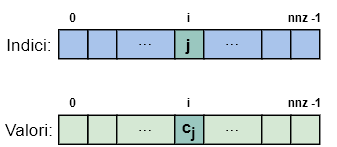
\includegraphics[scale=0.5]{Images/lazy_constraints}\\ 
  \caption{\footnotesize{Array lazy constraints}}
  \label{lazy_constraints} 
\end{center} 
\end{figure}
\subsection{Calcolo della soluzione}
Per ottenere la soluzione ottima del problema di ottimizzazione del problema correlato al modello definito in cplex, vengono utilizzate due fasi:
\begin{itemize}
\item{\textbf{Risoluzione del problema di ottimizzazione}\\
\begin{center}
\begin{tabular}{c}
\begin{lstlisting}[linewidth=120pt, basicstyle=\footnotesize\sffamily,]
CPXmipopt(env, lp);
\end{lstlisting}
\end{tabular}
\end{center}
\begin{table}[h]
\centering
\begin{tabular}{rl}
\textbf{env:} & {puntatore di tipo CPXENVptr alla struttura ENV}\\
& {precedentemente creata}\\
\textbf{lp:} & {puntatore di tipo CPXLPptr alla struttura LP}\\
& {precedentemente creata}\\
\end{tabular}
\end{table}
}
\item{\textbf{Ottenimento della soluzione}\\
\begin{center}
\begin{tabular}{c}
\begin{lstlisting}[linewidth=230pt, basicstyle=\footnotesize\sffamily,]
CPXgetx(env, lp, x, inizio, fine);
\end{lstlisting}
\end{tabular}
\end{center}
\begin{table}[h]
\centering
\begin{tabular}{rl}
\textbf{env:} & {puntatore di tipo CPXENVptr alla struttura ENV}\\
& {precedentemente creata}\\
\textbf{lp:} & {puntatore di tipo CPXLPptr alla struttura LP}\\
& {precedentemente creata}\\
\textbf{x:} & {puntatore a un vettore di double in cui verranno salvati}\\
\end{tabular}
\end{table}
\begin{table}[h]
\centering
\begin{tabular}{rl}
& {i valori delle variabili ottenuti dalla soluzione ottima}\\
\textbf{inizio:} & {primo indice della variabile di cui si vuole memorizzare}\\
& {ed analizzare il valore}\\
\textbf{fine:} & {indice dell'ultima variabile di cui si vuole memorizzare}\\
& {ed analizzare il valore}\\
\end{tabular}
\end{table}
Questa funzione salva in x tutte le variabili che hanno indice $i\in [inizio, fine]$ e quindi x deve essere un vettore di almeno $fine-inizio+1$ valori. Nel nostro programma, vengono analizzati i valori di tutte le variabili in gioco.\\
Per questo motivo \textbf{inizio=0} e \textbf{fine=num\_colonne - 1}\footnote{numero di variabili=CPXgetnumcols(env,lp);}\footnote{numero di vincoli=CPXgetnumrows(env,lp);}. In seguito il nostro programma analizza la correttezza della soluzione svolgendo la verifica su:
\begin{itemize}
\item{\textit{valori assunti dalle variabili}\\
ciascun $x_{i,j}$ assume valore $0$ o $1$ con una tolleranza di $\epsilon=10^{-5}$}
\item{\textit{grado di ciascun nodo}\\
il tour è composto al massimo da due archi che toccano lo stesso nodo}
\end{itemize}
}
\end{itemize}
\section{Parametri}
Con le seguenti funzioni è possibile modificare i parametri di impostazione di CPLEX, altrimenti impostati ai valori di default.
Nel caso in cui si tratti di parametri di tipo INT è necessario invocare:\\
\begin{center}
\begin{tabular}{c}
\begin{lstlisting}[linewidth=330pt, basicstyle=\footnotesize\sffamily,]     
CPXsetintparam(env, numero_parametro, nuovo_valore);
\end{lstlisting}
\end{tabular}
\end{center}
mentre se di tipo DOUBLE:\\
\begin{center}
\begin{tabular}{c}
\begin{lstlisting}[linewidth=330pt, basicstyle=\footnotesize\sffamily,]     
CPXsetdblparam(env, numero_parametro, nuovo_valore);
\end{lstlisting}
\end{tabular}
\end{center}
In entrambe le funzioni
\begin{table}[h]
\begin{tabular}{rl}
\textbf{env:} & {puntatore di tipo CPXENVptr alla struttura ENV}\\
& {di cui si vogliono cambiare i parametri}\\
\textbf{numero\_parametro:} & {intero corrispondente al parametro da modificare}\\
\textbf{nuovo\_valore:} & {nuovo valore (rispettivamente intero o double)}\\
& {del parametro}\\
\end{tabular}
\end{table}
\section{Costanti utili}
\begin{table}[h]
\begin{tabular}{|r|l|}
\hline
\textbf{CPX\_ON} & {1}\\ \hline
\textbf{CPX\_OFF} & {0}\\ \hline
\textbf{CPX\_INFBOUND} & {$\infty$}\\ \hline
\end{tabular}
\end{table}